% Switch between de/en and ids/tks as needed
\documentclass[de,ids]{fziartcl}
% \documentclass[en,tks]{fziartcl}
% \documentclass[de,ids]{fziartcl}
% \documentclass[en,ids]{fziartcl}


\usepackage[utf8]{inputenc}
\usepackage[ngerman]{babel}
\usepackage{csquotes}
\usepackage{fontenc}
\usepackage{graphicx}
\usepackage[comma,authoryear]{natbib}
\usepackage{float}
%\usepackage[backend=biber]{biblatex}
%\usepackage{underscore}


% You probably want to remove this and the \blindtext below
\usepackage{blindtext}

% Only needed if you use tikzpicture (you should!)
\usepackage{tikz,pgfplots}
\pgfplotsset{compat=1.9}
\usetikzlibrary{shapes.arrows,chains}

\bibliographystyle{apalike}
%\addbibresource{./example.bib}

\usepackage{listings}
\renewcommand{\lstlistingname}{Algorithmus}

\usepackage{color}

\definecolor{mygreen}{rgb}{0,0.6,0}
\definecolor{mygray}{rgb}{0.5,0.5,0.5}
\definecolor{mylightgray}{rgb}{0.9,0.9,0.9}
\definecolor{mymauve}{rgb}{0.58,0,0.82}

\lstset{ %
  backgroundcolor=\color{white},   % choose the background color; you must add \usepackage{color} or \usepackage{xcolor}
  basicstyle=\footnotesize\ttfamily,        % the size of the fonts that are used for the code
  breakatwhitespace=false,         % sets if automatic breaks should only happen at whitespace
  breaklines=true,                 % sets automatic line breaking
  captionpos=top,                    % sets the caption-position to bottom
  commentstyle=\footnotesize\ttfamily,    % comment style
  deletekeywords={...},            % if you want to delete keywords from the given language
  escapeinside={\%*}{*)},          % if you want to add LaTeX within your code
  extendedchars=true,              % lets you use non-ASCII characters; for 8-bits encodings only, does not work with UTF-8,
  frame=lines,
  float=hbt,
  framesep=2mm,	                   % adds a frame around the code
  keepspaces=true,                 % keeps spaces in text, useful for keeping indentation of code (possibly needs columns=flexible)
  %keywordstyle=\scfamily,       % keyword style
  keywordstyle=,       % keyword style
  language=Octave,                 % the language of the code
  otherkeywords={*,...},           % if you want to add more keywords to the set
  numbers=left,                    % where to put the line-numbers; possible values are (none, left, right)
  numbersep=5pt,                   % how far the line-numbers are from the code
  numberstyle=\tiny, % the style that is used for the line-numbers
  %numberstyle=\tiny\color{mygray}, % the style that is used for the line-numbers
  rulecolor=\color{black},         % if not set, the frame-color may be changed on line-breaks within not-black text (e.g. comments (green here))
  showspaces=false,                % show spaces everywhere adding particular underscores; it overrides 'showstringspaces'
  showstringspaces=false,          % underline spaces within strings only
  showtabs=false,                  % show tabs within strings adding particular underscores
  stepnumber=1,                    % the step between two line-numbers. If it's 1, each line will be numbered
  stringstyle=\color{mymauve},     % string literal style
  tabsize=2,	                   % sets default tabsize to 2 spaces
  title=\lstname                   % show the filename of files included with \lstinputlisting; also try caption instead of title
}


% Place your name here
\author{Dennis Nienhüser}

% You can override the date, if needed
% \date{21.11.2012}

\title{Eine beispielhafte Studie}

\begin{document}

\maketitle

\tableofcontents
\newpage

% Einleitung
\section{Einleitung} % 1 Seite
\subsection{Aufgabenstellung}
Ziel des diesjährigen Praktikum Mobile Roboter mit dem Thema \glqq Coffee to go\grqq war es, eine Tasse Kaffee,  welche auf einem Tisch platziert wurde mittels eines Roboterarms zu greifen, auf einem mobilen Roboter zu platzieren und diese, nach Transport durch selbigen, dann mittels eines zweiten Roboterarms wieder auf einen zweiten Tisch zu stellen.
Die Aufgabe unserer Gruppe war hierbei, die Tasse auf dem ersten Tisch zu lokalisieren, sie zu greifen und auf dem mobilen Roboter zu platzieren. % Daniel 0.2 Seiten
\subsection{Ausgangssituation}
Als Ausgangspunkt für die Realisierung der Aufgabe wurde uns sowohl diverse Hardware als auch Software zu Verfügung gestellt. So stand uns für das Greifen der Tasse ein UR5 Roboter von Universal Robots, welcher bereits auf einem Tisch befestigt wurde. Zur Lokalisierung der Tasse waren eine Kinect bzw. alternativ eine Intel Realsense Kamera verfügbar. Außerdem standen uns für die Entwicklung der Software sowohl vorkonfigurierte Rechner in Poolräumen, als auch ein an den UR5 Roboter angeschlossener Shuttle PC zur Verfügung. Als Grundlage für die zu entwickelnde Software dienten ROS Indigo bzw. Kinetic. % Daniel 0.2 Seiten
\subsection{Systemarchitektur}
\subsubsection{Hardware} % Robin 0.2 Seiten
Zur Erfüllung unserer Aufgabe wurden uns ein UR5 Roboterarm, ein Schunk PG70 und eine Microsoft Kinect zur Verfügung gestellt. Der UR5 wurde für uns in der linken Ecke am Tisch montiert und der PG70 über ein Verbindungsstück mit dem Roboterarm verbunden. Zum Greifen der Tasse mussten wir selbst modellierte Greifer anfertigen lassen, welche passgenau am PG70 angebracht wurden. Mit Hilfe von Bosch Elementen haben wir die Kinect Kamera in der unteren Ecke des Tisches in einer Höhe von einem Metern über der Tischplatte platziert. Diese Höhe war notwendig, um die linke, obere und rechte Ecke des Tisches, sowie den Bereich direkt links unterhalb des UR5 einfangen zu können. Die drei Ecken wurden als Orientierungspunkte der Kamerakalibrierung benutzt. Den Aufbau der Hardware kann man in Abbildung \ref{Hardware} sehen.
\newline
Weiterhin wurde festgelegt, dass sich der Turtlebot im Bereich direkt links unterhalb des Roboterarms zur Tassenübergabe platzieren soll.
\begin{figure}
	\centering
	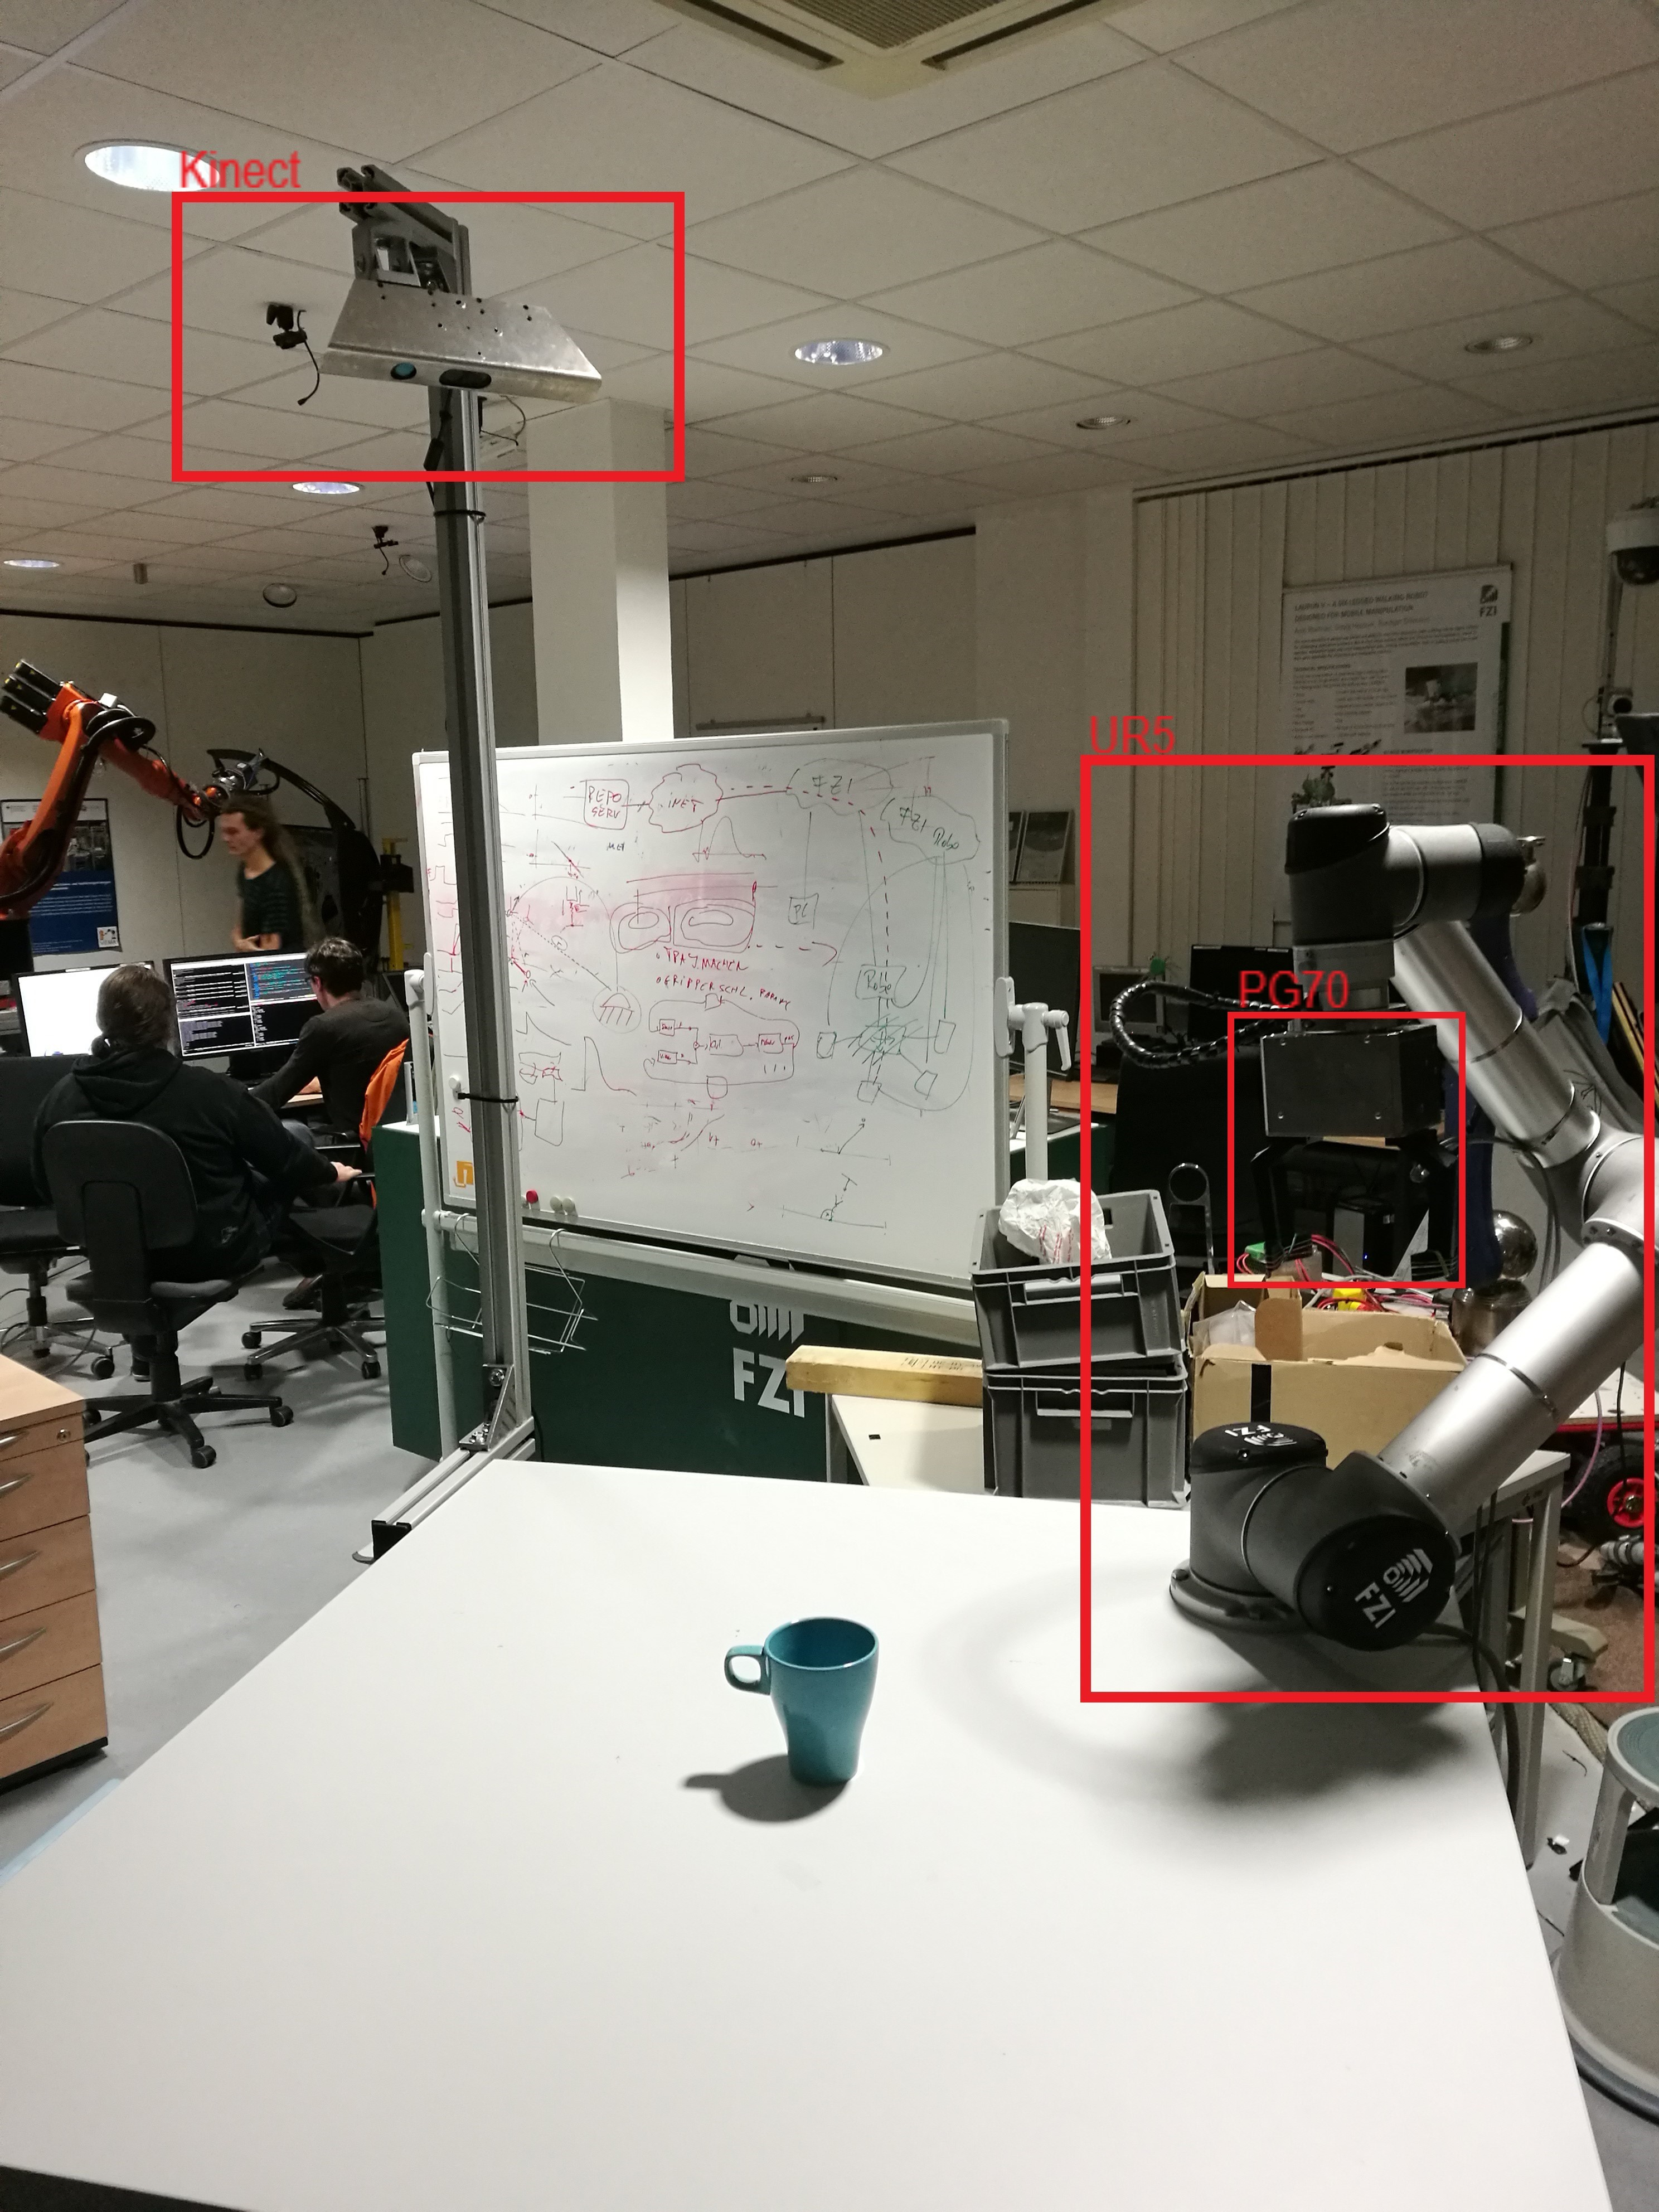
\includegraphics{images/Hardware-Aufbau_Beschriftung.pdf}
	\caption{Aufbau der Hardware: Kinect Kamera (links oben), UR5 (rechts), PG70 (am Ende des UR5)}
	\label{Hardware}
\end{figure}
\subsubsection{Software}
Der Softwareteil besteht grundsätzlich aus vier Komponenten. Die Lokalisierungskomponente ermöglicht die Detektion der Tasse und des Turtlebots. Sie stellt zudem diverse Werkzeuge zur automatischen Kamerakalibrierung, Poseschätzung der Tasse, Manipulation der Punktwolken und  Annotation der Datensätze zur Verfügung. Die Bahnplanungskomponente führt die Bahnplanung des Roboterarms zwischen der erkannten Tasse und dem erkannten Turtlebot aus. Die Greifkomponente steuert den Fingerabstand, um die erkannte Tasse zu greifen bzw. die Tasse auf den erkannten Turtlebot zu legen. Letztendlich dient die High-Level-Steuerung zur Koordination der verschiedenen Softwarekomponenten und bietet die Schnittstelle zur Kommunikation mit dem zentralen State Manager der drei Gruppen an.\\
 % Vorbereitung Yassine. Verifizieren Sonntag zusammen. 0.2 Seiten
\subsection{Arbeitspakete} % 0.2 Seiten
Die Lösung der gestellten Aufgabe haben wir in folgende Arbeitspakete unterteilt:

\begin{table}[H]
\scalebox{0.7}{
\begin{tabular}{|p{5cm}|p{5cm}|p{5cm}|} \hline
Hauptaufgabe & Arbeitspaket & Zuständigkeit \\ \hline
Bilderkennung &  &  \\ \hline
& Erstellung der Softwarearchitektur für die Bilderkennung & Daniel Klitzke \\ \hline
 & Tassendetektion mit FCN & Daniel Klitzke, Yassine El Himer \\ \hline
 & Tassendetektion Segmentierung + Neuronale Netze & Daniel Klitzke \\ \hline
 & Tassendetektion SVM + HOG Features & Daniel Klitzke \\ \hline
 & Segmentierung der Tasse aus der Punktwolke & Daniel Klitzke \\ \hline
 & Erkennung der Tassenorientierung & Daniel Klitzke \\ \hline
 & Evaluation von YOLO als Alternative für die Tassendetektion & Yassine El Himer \\ \hline
 & Turtlebotdetektion SVM + HOG Features & Yassine El Himer \\ \hline
 & Segmentierung des Turtlebot aus der Punktwolke & Yassine El Himer \\ \hline
 & Automatische Kamerakalibrierung & Daniel Klitzke \\ \hline
 Bahnplanung \& Greifen & & \\ \hline
 & Aufsetzen der Simulation & Robin Weitemeyer \\ \hline
 & Modellierung der Roboterumgebung & Robin Weitemeyer \\ \hline
 & Konfiguration von MoveIt & Robin Weitemeyer \\ \hline
 & Bahnplanung mit MoveIt & Robin Weitemeyer \\ \hline
 & Modellierung eines Greifers & Florian Dreschner \\ \hline
 & Ansteuerung und Verwendung des UR5 & Robin Weitemeyer \\ \hline
 & Ansteuerung und Verwendung des Greifers & Florian Dreschner \\ \hline
 & Implementierung der Planungslogik & Robin Weitemeyer  \\ \hline
 High-level Steuerung \& Kommunikationsschnittstellen & & \\ \hline
 & Bestimmung und Evaluierung der Schnittstellen & Yassine El Himer, Florian Dreschner  \\ \hline
 & Implementierung des Managers & Florian Dreschner  \\ \hline
 Sonderaufgaben & & \\ \hline
 & Hardwareaufbau & Robin Weitemeyer \\ \hline
 & High-level Steuerung & Yassine El Himer \\ \hline
 & Kommunikation & Florian Dreschner \\ \hline
 & Dokumentation & Daniel Klitzke \\ \hline
 \end{tabular}
}
 \caption{Die Einteilung der Arbeitspakete.}
 \label{tab:work-packages}
\end{table} % Daniel

% State-of-the-art
\section{State of the Art} % 1.5 Seiten
\subsection{Bilderkennung}
In diesem Abschnitt sollen die für unsere Aufgabenstellung relevanten Themen aus der aktuellen Forschung vorgestellt werden.

Die Lokalisierung der Tasse lässt sich auf vielfältige Art und Weise realisieren. Eine Strategie, die wir auch in unserem Ansatz verfolgen, ist es die Tasse in den Bilddaten zu detektieren und die exakten Abmessungen anschließend aus der Punktwolke zu berechnen. Aus diesem Grund ist für uns vor allem das große Feld der Objekterkennung interessant. Hier zeichnet sich in den letzten Jahren deutlich der Trend hin zu Verfahren des maschinellen Lernens, insbesondere des Deep Learnings, ab. Vorangetrieben wird dies insbesondere durch die Entwicklung leistungsfähiger Hardware, insbesondere von GPUs, sowie der Verfügbarkeit von großen Trainingsdatensätzen. Deep-Learning basierte Ansätze wurden in folgenden für uns relevanten Bereichen bereits eingesetzt und übertrafen bisherige Ansätze deutlich.

\paragraph{Bild Klassifikation}
Ein für uns relevanter Bereich ist die Bild Klassifikation. Das Ziel hierbei ist es in Bildern präsente Objekte korrekt zu klassifizieren. Aktuelle Ansätze wie setzen hierbei auf der Verwendung von Convolutional Neural Networks (CNNs). Wichtige Publikationen sind u.A. \cite{He.2016} und \cite{Szegedy.20151211}

\paragraph{Objekt Detektion}
Das Ziel bei der Objekt Detektion ist es, Objekte einer bestimmten Klasse in einem Bild zu detektieren. Für die Klassifikation von Bildern entworfene Neuronale Netze werden häufig auch für die Objekt Detektion eingesetzt, indem sie mit anderen Verfahren kombiniert werden. Für konkrete Beispiele zur Objekt Detektion mittels Deep Learning siehe auch \cite{Dai.20160621} und \cite{Ren.2017}. 

\paragraph{Semantische Segmentierung}
Insbesondere im Bereich des autonomen Fahrens gewannen Ansätze zur Semantischen Segmentierung in den letzten Jahren stark an Popularität. Das Ziel einer semantischen Segmentierung ist es, jedem Pixel eines Eingabebildes eine Objektklasse zuzuordnen. Realisiert wird dies zumeist über sogenannte Fully Convolutional Neural Networks. Wichtige Publikationen im Bereich der semantischen Segmentierung sind u.A. \cite{Shelhamer.2017}, \cite{Chen.20170512} und \cite{Badrinarayanan.2017}.

Neben den vorgestellten Deep Learning Ansätzen kann es auch durchaus angebrachter sein andere Verfahren des Maschinellen Lernens zu verwenden. Gründe hierfür könnten unter anderem die Knappheit von Trainingsdaten, limitierte Hardware Resourcen als auch aufgabenspezifische Eigenheiten sein. Um insbesondere im Bezug auf limitierte Hardware Resourcen und die Knappheit von Trainingsdaten Abhilfe zu schaffen kann es insbesondere bei überschaubaren Problemstellungen gerechtfertigt sein auch flache Klassifikatoren einzusetzen. Ein populärer Vertreter der flachen Klassifikationsverfahren sind die Support Vector Machines. Diese wurden in \cite{Dalal.2005} erstmals in Kombination mit HOG Features für die Detektion von Personen in Bilddaten eingesetzt.

Eine Alternative wäre es gewesen, die Tasse nicht mithilfe der Bilddaten, sondern mithilfe der Punktwolke zu detektieren. Auch hier existieren Deep Learning basierte Ansätze wie z.B. \cite{Maturana.2015} oder \cite{Engelcke.20170305}. % Daniel 0.75 Seiten
\subsection{Bahnplanung \& Greifen}
Im Bereich der Bahnplanung genießen auf Abtastung basierende Algorithmen wie \textit{probabilistic roadmap} (PRM) oder \textit{rapidly-exploring random tree} (RRT) große Beliebtheit. Was nicht zuletzt an ihrer asymptotischen Optimalität, siehe \cite{SamplingAlgos}, liegt.
\newline
Die PRM-Planungsmethode, siehe \cite{PRM}, besteht aus zwei Phasen:
\begin{enumerate}
	\item Learning-Phase
	\item Query-Phase
\end{enumerate}
In der Learning-Phase wird ein kollisionsfreier Graph im Konfigurationsraums des Roboters erstellt, indem zufällige Punkte im Raum auf Kollision untersucht wird und anschließend mit Hilfe eines lokalen Pfadplaners mit dem bestehenden Graph, ebenfalls kollisionsfrei, verbunden wird. In der Query-Phase wird durch einen Graphsuchalgorithmus ein Pfad vom Anfangs- zum Zielpunkt bestimmt.
\newline
Die RRT-Methode, siehe \cite{RRT}, benötigt keine Learning-Phase. Zwar werden auch hier zufällig Punkte im Konfigurationsraum ausgewählt und auf Kollision mit der Umgebung geprüft, der Aufbau des Graphes, welcher die Form eines Suchbaums besitzt, geschieht jedoch für jede Pfadanfrage von Neuem. Somit benötigt eine Suchanfrage bei der RRT-Methode potentiell länger im Vergleich zu PRM, der Graph berücksichtigt jedoch auch dynamische Objekte, deren Position sich in der Umgebung verändern kann.
\newline
RRT-Connect, siehe \cite{RRTConnect}, ist eine Erweiterung von der RRT-Planungsmethode. Hier werden zwei Suchbäume gleichzeitig aufgebaut. Einer beginnt vom Startzustand, der andere vom Zielzustand. Dabei wird eine greedy-Heuristik verwendet, um die Wahrscheinlichkeit zu erhöhen, dass sich die beiden Bäume aufeinander zubewegen. Nach einer vorgegebenen Anzahl von Iterationen wird versucht, die beiden Bäume direkt zu verbinden.
 % Robin 0.75 Seiten

% Arbeitsbericht
\section{Arbeitsbericht} % 3 Seiten
\subsection{Bilderkennung}
\subsubsection{Tassenerkennung}
\paragraph{Allgemein}
Für die Tassenerkennung wurden keinerlei ROS Pakete verwendet. Stattdessen wurden die einzelnen Komponenten in Python selbst implementiert. Die am häufigsten zur Hilfe genommenen Bibliotheken sind unter anderem:
\begin{itemize}
\item NumPy (Effizienter Umgang mit Matrizen und Vektoren)
\item scikit-image (Bildverarbeitung)
\item scikit-learn (Algorithmen für Maschinelles Lernen)
\item Keras (High-level API für die Erstellung von Neuronalen Netzen)
\item Matplotlib (Visualisierung)
\end{itemize}

\paragraph{Detektion der Tasse in den Bilddaten}
Für die Detektion der Tasse in den Bilddaten wurden eine Reihe von Ansätzen getestet, bevor die finale Lösung feststand.

Zunächst war der Plan die Tasse mittels eines Fully Convolutional Neural Network aus den Bilddaten zu segmentieren. Als Basisstruktur wurde hierfür die Architektur des Resnet50 Netzes verwendet. Die Eingabe für das Netz stellt ein RGB Bild dar und es liefert als Ausgabe zwei Feature Maps, welche die Wahrscheinlichkeiten für die Zugehörigkeiten der Pixel des Eingabebildes zu den Klassen \glqq Tasse\grqq bzw. \glqq Keine Tasse\grqq enthalten. Trainiert wurde auf den Microsoft COCO Datensatz unter Nutzung von GPU Kapazitäten bei Amazon Webservices. Der Ansatz wurde letztendlich verworfen, da es sich herausstellte dass das Netz zu überdimensioniert für die Segmentierung einer Klasse aus einem RGB Datensatz ist und nicht genügend Trainingsdaten zur Verfügung standen.

Der zweite getestete Ansatz basierte auf der Segmentierung des Bildes in eine Menge von Segmenten sowie einer Klassifizierung durch ein Neuronales Netz. Das Bild wird hierfür zunächst mittels des SLIC Algorithmus in eine Menge von Segmenten zerlegt. Diese Segmente werden dann unter Einbeziehung eines gewissen Kontextfensters dem Neuronalen Netz zur Klassifikation übergeben. Jedem Segment wird entweder als \glqq Tasse\grqq oder \glqq Keine Tasse\grqq klassifiziert. Das Ergebnis einer Vorhersage mit dem beschriebenen Algorithmus ist in Abbildung \ref{fig:patches_prediction_result} abgebildet.

\begin{figure}
    \centering
    \begin{minipage}{0.45\textwidth}
        \centering
        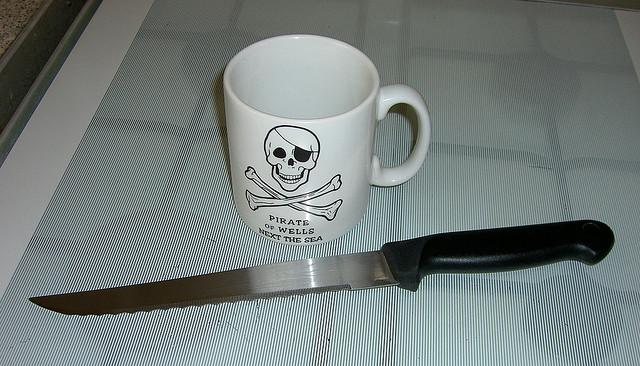
\includegraphics[width=0.9\textwidth]{images/cup_patches.jpg} % first figure itself
        \caption{Eingabe für das Neuronale Netz zur Segment Klassifikation \label{fig:patches_prediction}}
    \end{minipage}\hfill
    \begin{minipage}{0.45\textwidth}
        \centering
        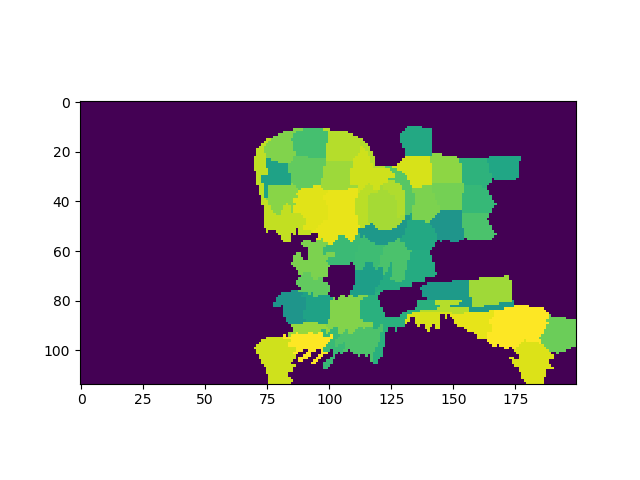
\includegraphics[width=0.9\textwidth]{images/cup_patches_prediction.png} % second figure itself
        \caption{Vom Netz ausgegebene Wahrscheinlichkeiten \label{fig:patches_prediction_result}}
    \end{minipage}
\end{figure}

Der dritte gewählte Ansatz wurde letztendlich auch in das fertige System übernommen und basiert auf einer SVM welche Bildsegmente, die mithilfe eines Sliding Window Ansatzes gewonnen werden klassifiziert. Details zu diesem Ansatz werden im Abschnitt \ref{4-1-1_gesamtsystem_bilderkennung_tassenerkennung} näher erläutert.

\paragraph{Segmentierung der Tasse in der Punktwolke}
Nachdem die Tasse in den Bilddaten detektiert wurde wird sie mittels eines Clustering Algorithmus aus den Bilddaten segmentiert. Hierbei traten keinerlei Komplikationen auf. Der Ansatz wird ebenfalls in \ref{4-1-1_gesamtsystem_bilderkennung_tassenerkennung} beschrieben.

\paragraph{Erkennung der Tassenorientierung}
Hier wurden zwei verschiedene Ansätze implementiert wovon letztendlich einer für das finale System ausgewählt wurde. Der erste Ansatz basiert auf dem RANSAC Algorithmus. Zunächst wird die Punktwolke der Tasse auf die x-y-Ebene projiziert und deren Zentrum bestimmt. Anschließend wird in jeder Iteration des Ransac Algorithmus ein zufälliger Punkt ausgewählt und eine Linie durch selbigen und das Zentrum der Tasse gelegt. Es wird die Konfiguration mit den meisten Inliern als Richtung des Tassengriffs ausgewählt. Es stellte sich hierbei heraus, dass die zum Tassengriff gehörigen Punkte im Vergleich zu den restlichen Punkten so wenig ins Gewicht fallen dass so keine zuverlässige Schätzung möglich war.
Der zweite Ansatz basiert auf dem Local Outlier Factor Schätzer und erwies sich als deutlich robuster als der zuvor beschriebene Ansatz. Er wird in \ref{4-1-1_gesamtsystem_bilderkennung_tassenerkennung} näher beschrieben. % Daniel 1 Seiten
\subsubsection{Turtleboterkennung}
\paragraph{Allgemein}
Für die Turtleboterkennung wurden keine ROS Pakete verwendet. Die verwendete Bibliotheken sind unter anderem NumPy, openCV, scikit-image, scikit-learn, Matplotlib.

\paragraph{Detektion des Turtlbots in den Bilddaten}
Die erste Überlegung war, das Turtlebot anhand eines Convolutional neural Networks zu erkennen. Mangels an Datensätze, die annotierte Bilder von der Klasse \textit{Turtlebot}\ in unterschiedlichen Kontexten beinhalten, wurde dieser überwachte Ansatz verworfen.

Eine günstigere aber robuste Alternative war ein auf einer SVM basiertes Model, das im Vergleich zu CNNs weniger annotierte Daten benötigt, um letztendlich die Stützvektoren zu finden. Nachdem ein Datensatz von verschiedenen annotierten Posen des Turtlebots in einer Szene mithilfe der Kinect erstellt und segmentiert wurde, wurde die SVM auf unteschiedlichen negativen und positiven Patches trainiert. Mehr zu diesem Ansatz wird im Abschnitt
\ref{4-1-2_gesamtsystem_bilderkennung_turtlebotkennung} detailliert.

Über den in das System übernommene Ansatz hinaus wurden noch zwei anderen Ansätze getestet. Im folgenden fassen wir sie kurz zusammen:

Der erste getestete Ansatz basierte sich auf das Template-Matching. Hier wurde ein Bild von der obigen Seite des Turtlebots aufgenommen und als Schablone verwendet. Diese wurde unterschiedlich skaliert und rotiert, um anhand einer Brute-Force-Suche das in der Szene gesuchte Turtlebot anzupassen.

Der zweite getestete Ansatz war ein Feature-Matching-Verfahren und erfolgte in zwei grundlegenden Schritten: Das Finden repräsentativer Bildmerkmale in den Bildern des Turtlebots und Das Zuordnen dieser mit denen eines Turtlebots in der Szene. Dabei wurde ORB (Oriented FAST and Rotated BRIEF) als effiziente und freie alternative zu SIFT und SURF verwendet. Mittels einer mit RANSAC linearen Regression der zugerodneten Keypoints und Deskriptoren von jeweils Turtlebot und Szene wurde die Homographie Matrix berechnet, um letztendlich eine Perspektivische Projektion des Turtlebots in der Szene zu realisieren. Wegen der niedrigen Auflösung der Kinect lieferte dieser Ansatz meistens unangemessene Ergebnisse.

\paragraph{Segmentierung des Turtlebots in der Punktwolke}
Aus der Detektion des Turtlebots in einem Bild werden die \(x\) und \(y\) Koordinate im Weltkoordinatensystem gewonnen. Die \(z\) Koordinate ist durch die Punktwolke zu bestimmen. Ein naïves Verfahren war, die Punkte aus der Wolke zu nehmen, die zwischen einer Tiefe von der Höhe des Turtlebots und der maximalen von der Kinect gelieferten Tiefe.
Werden die \(x\),\(y\) und \(z\) Koordinate kombiniert, wird das 3D-Bounding-Box des Turtlebots bestimmt. % Yassine 0.25 Seiten
\subsubsection{Automatische Kamerakalibrierung}
So wie auch die Tassenerkennung wurde auch die Kalibrierung der Kamera ohne die Verwendung von fertig verfügbaren ROS Paketen realisiert. Es wurden zwei Ansätze realisiert wobei sich der als zweites implementierte Ansatz als deutlich robuster und genauer erwiesen hat und deshalb in das Gesamtsystem aufgenommen wurde.
Der zunächst implementierte Algorithmus basiert auf der Segmentierung der Tischplatte aus der Punktwolke. So wird als erster Schritt die Tischebene mittels des RANSAC Algorithmus aus der Punktwolke segmentiert. Der berechnete Normalenvektor der Eben wird anschließend dazu verwendet um die Tischplatte so zu rotieren, dass sie parallel zur x-y-Ebene ist. Daraufhin wird die minimale Bounding Box der Tisch Punktwolke im 2 Dimensionalen Raum berechnet und als Tischfläche angenommen. Es stellte sich beim testen des Algorithmus heraus, dass die Methode zwar schnell ist, jedoch zu ungenaue Ergebnisse liefert. Die Ungenauigkeiten waren wohl vor allem darauf zurückzuführen, dass die Punktwolke an den Ecken der Tischplatte einige Löcher aufwies und die Bounding Box so nicht den eigentlichen Umriss des Tisches wiedergab. Neben den Ungenauigkeiten bei der Tischdetektion ergab sich ein weiterer Nachteil aus den zur Ausführung des RANSAC Algorithmus verwendeten Python Bindings für PCL. So wurden diese, obwohl von der PCL Webseite verlinkt, augenscheinlich nicht mehr sehr aktiv gewartet und waren doch sehr unvollständig und teilweise fehlerhaft. Dies weckte zusätzlich den Wunsch die entsprechende Bibliothek aus dem Projekt zu entfernen.
So wurde schlussendlich ein zweite Ansatz implementiert. Dieser basiert auf der Detektion der Tischkanten aus den Bilddaten sowie einer anschließenden Segmentierung der die Tischkanten repräsentierenden Geraden in der Punktwolke. Beim testen des Ansatzes erwies sich dieser als deutlich genauer als die vorher implementierte Methode und auch die RANSAC Implementierung konnte mit geringem Mehraufwand, der durch die Implementierung einer geeigneten BaseEstimator Klasse entstand, durch die Implementierung von scikit-learn ersetzt werden. Die Details des schlussendlich implementierten Algorithmus sind in \ref{4-1-2_gesamtsystem_bilderkennung_automatische_Kamerakalibrierung} beschrieben. % Daniel 0.5 Seiten
\subsection{Bahnplanung \& Greifen}
\subsubsection{Bahnplanung}
Die Aufgabe der Bahnplanung war es, den PG70 unter Verwendung des UR5 zur Position der Kaffeetasse zu manövrieren, um diese zu greifen und anschließend sicher und ohne das Verschütten jeglicher Flüssigkeit auf den Turtlebot abzustellen. Dabei gab es mehrere Problem, die es zu bewältigen gab.
\newline
Zum einen musste dem Roboterarm gesagt werden, wo sich die Tasse bzw. der Turtlebot befindet und wie er die beiden Ziele ansteuern soll. Dabei musste sowohl eine Selbstkollision, als auch eine Kollision mit der Umgebung vermieden werden. Des Weiteren war es auf der Strecke von der Kaffeetasse zum Turtlebot notwendig, dass die Tasse ihre aufrechte Orientierung beibehält, damit der Kaffee bei dem Transport nicht verschüttet wird.
% Für die Lokalisierung war es außerdem hilfreich, dass der UR5 sich, wenn er nicht gerade die Tasse befördert, in einer Home-Konfiguration befindet, in der er nicht unnötigerweise in den Bildbereich des Tischen hineinragt und somit die Lokalisierung erschwert oder die Tasse sogar völlig verdeckt.
\newline
Um diese Aufgabe zu erfüllen und die dabei auftretenden Probleme zu lösen, hatten wir uns zwei Optionen herausgesucht, zwischen denen wir uns entscheiden mussten:
\begin{enumerate}
	\item Die Bahnplanung mit dem Motion Planning Framework MoveIt \cite{MoveIt} realisiern.
	\item Die Bahnplanung mit der FZI-hauseigenen Motion Pipeline \cite{FZIPipeline} realisiern.
\end{enumerate}
MoveIt ist eine Stage of the Art Software zur Steuerung von Robotern. Sie beinhaltet verschiedene Lösungen der inversen Kinematik (IK), unterschiedliche Planer zur Trajektorienerstellung und Optimierungsmöglichkeiten der gefundenen Trajektorien. MoveIt ist mit all seinen Möglichkeiten und Anwendungsgebieten sehr umfangreich und komplex. Dafür existieren jedoch ausführliche Dokumentationen und Tutorials, sowie eine aktive Community, die sich bei Fragen und Probleme untereinander zu Rat steht.
\newline
Die FZI-eigene Motion Pipeline ist ein Framework zur einfachen Ausführung von Trajektorien auf bekannten Kinematiken. Dank einer rqt-GUI ist es besonders benutzerfreundlich, zum Beispiel Bahnen für einen Roboterarm zu lernen. Diese Trajektorien können dann gespeichert werden und müssen nur noch vor der Ausführung geladen werden. Auch die FZI Motion Pipeline besitzt eine Dokumentation, welche im Vergleich zu MoveIt allerdings weniger umfangreich ist.
\newline
Letzten Endes haben wir uns für den Einsatz von MoveIt entschieden. Denn obwohl dieses Framework für unsere Anwendungszwecke übermächtig ist und aufgrund der Komplexität eine länger Einarbeitsphase benötigt, wollten wir uns trotzdem im Bereich der Bahnplanung keine Grenzen setzen. MoveIt schien uns daher als das Mittel der Wahl.
\newline
Der erste Schritt bei der Integrierung von MoveIt in unser Projekt war es daher, das Framework für unseren genauen Roboteraufbau zu konfigurieren. Unter Verwendung des MoveIt Setup Assistant \cite{MoveItAssistant} erzeugten wir uns, mit Hilfe unseres selbst erstellten URDF-Modells, unser eigenes ROS-Paket mit allen Konfigurations- und Launch-Dateien, die wir für die Benutzung von MoveIt auf unserer Hardware benötigten.
%Da wir die Bahnplanung in Python implementierten mussten wir außerdem noch das ROS-Paket "`Moveit_Commander"' \cite{MoveItCommander} zu unserem Projekt hinzufügen.
\newline
Zur Bahnplanung in MoveIt verwendeten wir Planer aus der Open Motion Planning Library (OMPL) verschiedene Planner, wobei wir uns Am Ende für den RRTConnectDefault entschieden. Dieser implementiert den RRT-Connect Algorithmus und lieferte uns die zuverlässigsten Ergebnisse. Bei den IK-Implementierungen gab es keine beobachtbaren Unterschiede.
\newline
Für die eigentliche Bestimmung der Trajektorie des UR5 stellt MoveIt zwei Methoden zur Verfügung.
\begin{enumerate}
	\item Bahnplanung vom momentanen Zustand zur Zielpose.
	\item Bahnplanung vom momentanen Zustand über eine Liste von Zielposen.
\end{enumerate}
Bei der ersten Variante wird nur der momentane Zustand des Roboters gesetzt. Anschließend wird mit der Methode \textit{set\_target\_pose} die Zielpose gesetzt und mit \textit{plan} die Bewegung geplant. Die zweite Methodik basiert auf der Bahnplanung über mehrere Wegpunkte. Die Methode \textit{compute\_cartesian\_path} bestimmt dabei aus mehreren Posen eine Trajektorie. Wir entschieden uns schließlich für die zweite Variante, da diese ohne Pfad-Constraints und weitere Optimierungsschritte für unsere Aufgabe optimale Bahnen bestimmte und auch die Ausrichtung der Tasse beibehielt.
 % Robin 1 Seite
\subsubsection{Greifen}
Ein weiterer Teil der Aufgabe befasste sich mit dem Greifen der Tasse. Dafür steht der Greifer Schunk PG70 zur Verfügung, sowie ein 3D-Drucker zur Erstellung von Fingern. Zu Beginn wurden zwei Griffvarianten in Betracht gezogen: 1) Seitliches Greifen und 2) Greifen von oben. Während seitliches Greifen natürlicher erscheint, erwies sich die Planung für einen Griff der Tasse von oben als einfacher. Um keine Variante vorzeitig auszuschließen, wurde ein Fingermodell mit zwei möglichen Griffflächen erstellt, eine Fläche am Ende des Fingers, sowie eine Ausbuchtung am Schaft des Fingers. Die Fläche am Endes des Fingers führte zu genau zwei Kontaktpunkten zwischen der Tasse und dem Endeffektor. Die Tasse wurde sehr instabil gehalten und neigte zu Schaukeln bei schnelleren Bewegungen. Desweiteren reichte die Reibung zwischen Kunststoff und Ton nicht für einen festen Griff aus.

Aus diesem Grund wurde die Anzahl der Kontaktpunkte durch eine eckige Ausbuchtung von zwei auf vier verdoppelt. Bei ersten Tests mit der eigentlichen Hardware wurde ein weiteres Problem erkannt: Der Gesamthub des Greifers ist geringer als der durchschnittliche Durchmesser der Tasse. Daher konnte zuerst nur eine von zwei Tassen gegriffen werden, außerdem beschränkte sich die Pufferzone auf weniger als 1cm pro Fingerbacke. Die ersten Ergebnisse aus der Bilderkennung legte eine deutliche Verbreitung der Griffbreite nahe, um Ungenauigkeiten bei der Approximation der Tasse auszugleichen.

Die folgende Generation an Fingern vergrößerte die Griffbreite um 4cm durch \glqq Nach-hinten\grqq -Lagerung jeder Backe. Zusätzlich wurde der Schaft verlängert und erhielt eine ähnliche kantige Ausbuchtung, wie bereits das Ende des Fingers. Diese Änderung vergrößerte den Arbeitsbereich des Roboters, den Sicherheitsabstand zum Tisch und die Kontaktfläche der Tasse am Schaft des Fingers.

Bei einem weiteren Versuch wurde durch einen Konfigurationsfehler zu tief unter die Kante der Tasse eingetaucht, was in letzter Konsequenz zum Brechen eines Fingers führte. Um dieses Problem bei einer weiteren Iteration kategorisch auszuschließen, wurde die Verschiebung des Schaftes an den Montagebereich gelegt, eine abfallende Kante in Richtung Ende des Fingers konstruiert und die Gesamtlänge von 12cm auf 11cm reduziert. Außerdem wurde die Druckrichtung von Horizontal auf Vertikal verändert, um die Stabilität zu erhöhen.

Zusätzlich wurden zwei Varianten für eine bessere Reibung getestet: 1) Arbeitshandschuh und 2) Haushaltsgummi. Aus dem Handschuh wurden zwei Finger entfernt und mit doppelseitigem Klebeband auf dem gedruckten Finger befestigt. Der Grip zwischen Finger und Tasse erhöht sich, jedoch ist die hinzugefügte Schicht dünn, weshalb der Finger sich bei erhöhtem Druck verbiegt. Zur Vermeidung wird eine dickere Schicht zwischen Finger und Tasse benötigt. Haushaltsgummis in einem X-Muster erwiesen sich als besser geeignet, da sie mehr Reibung und eine dickere Schicht bieten.

\begin{figure}
    \centering
    \begin{minipage}{0.45\textwidth}
        \centering
        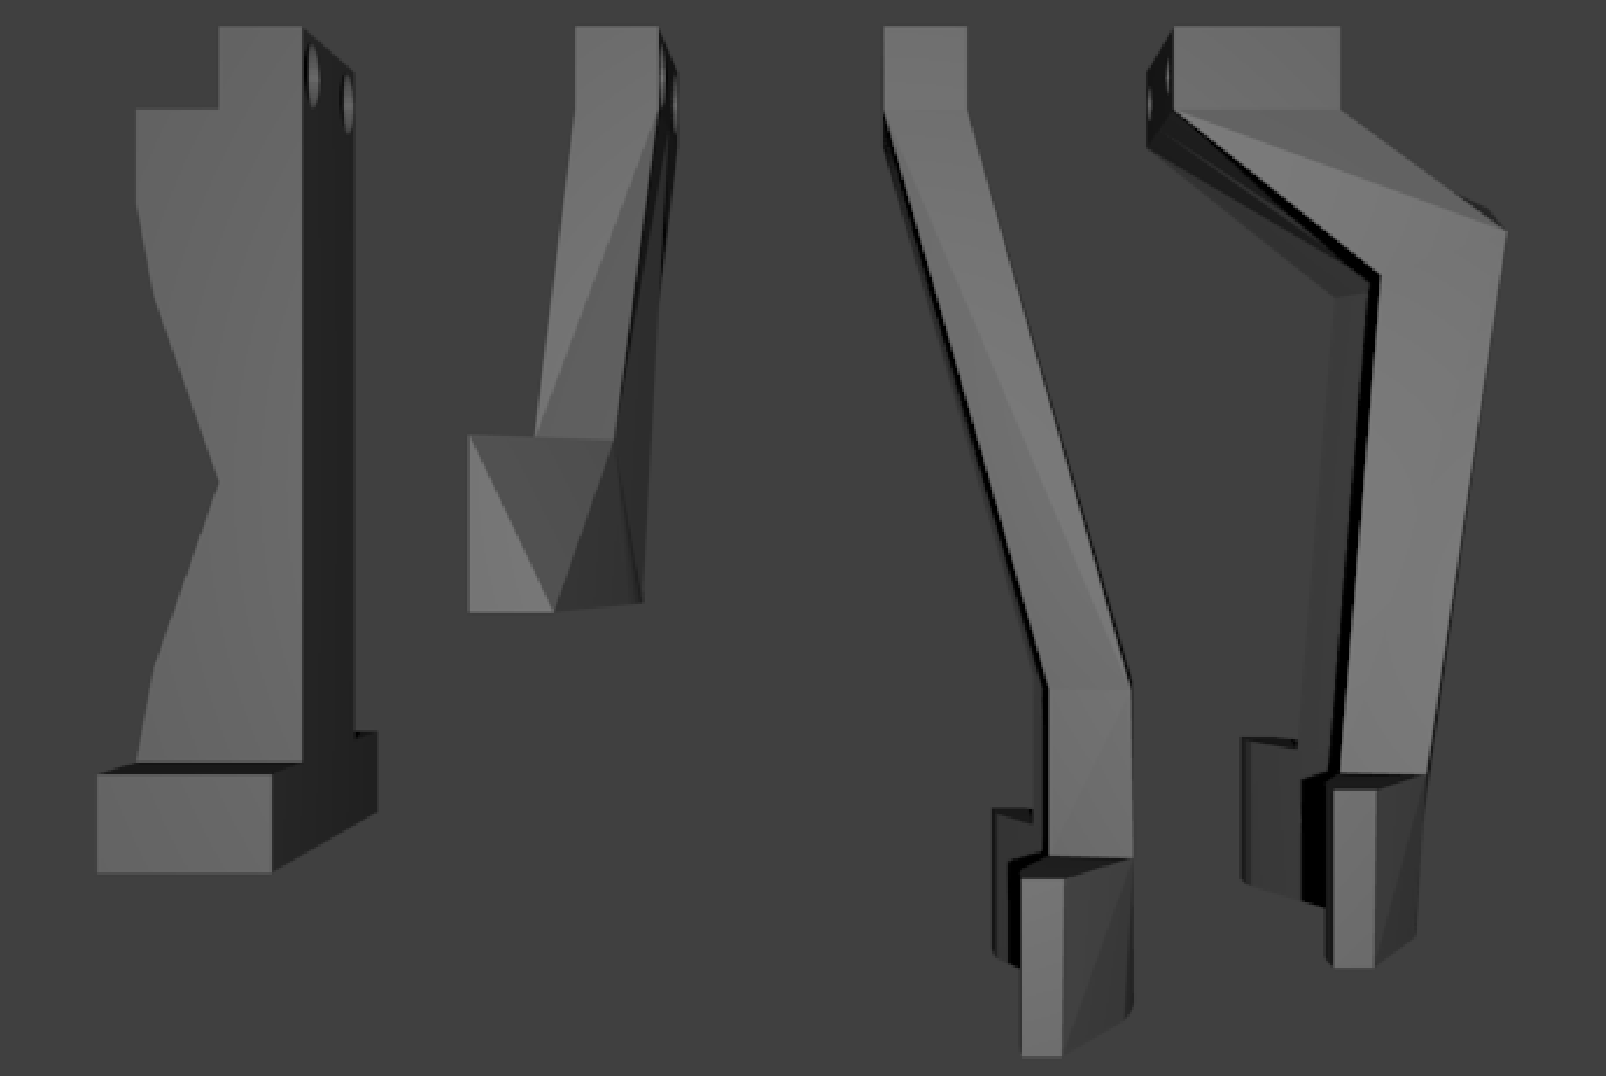
\includegraphics[width=0.9\textwidth]{images/finger_evolution.png} % first figure itself
        \caption{Evolution des Fingers}
    \end{minipage}\hfill
    \begin{minipage}{0.45\textwidth}
        \centering
        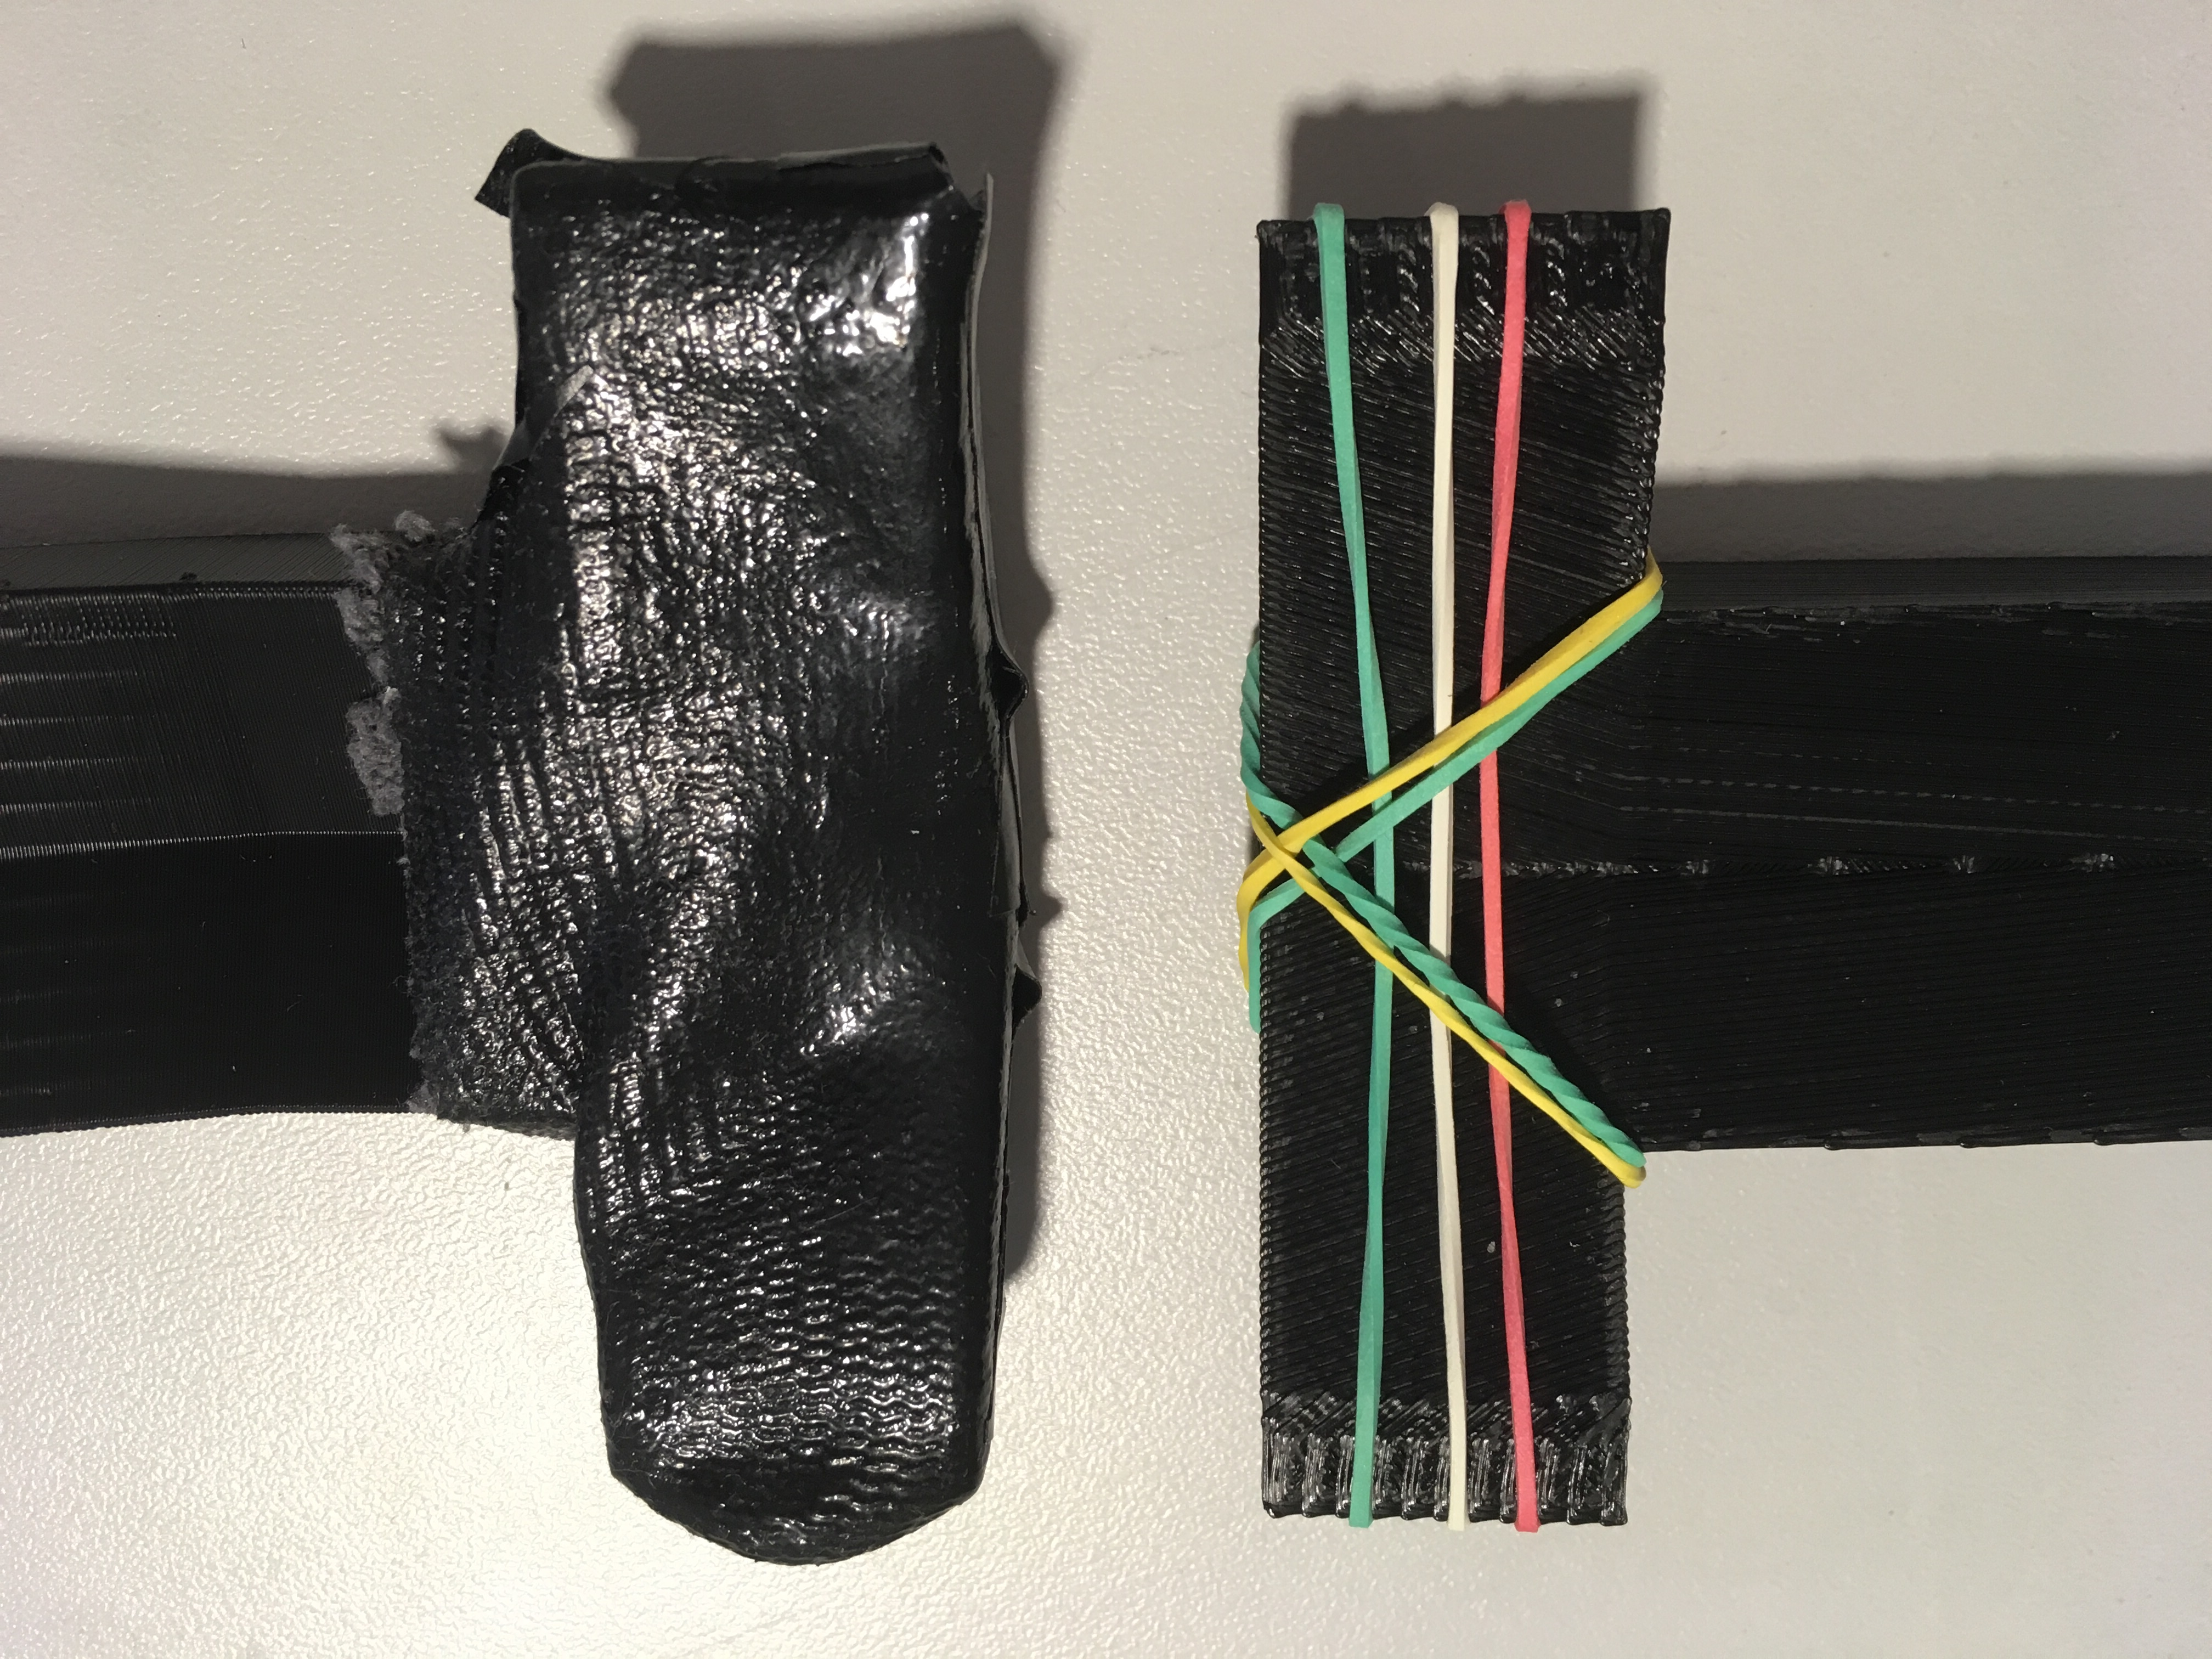
\includegraphics[width=0.9\textwidth]{images/finger_tip.JPG} % second figure itself
        \caption{Erhöhter Grip}
    \end{minipage}
\end{figure}

Abhängig von der Tasse wurden verschiedene Konstanten für die Breite der Finger empirisch getestet. Zur Vereinfachung gehen wir nun von genau einem Tassenmodell mit einer festen Breite aus. Anfangs wurde mit einem Fingerabstand von 9mm gegriffen, jedoch lässt sich dieser Wert zugunsten der Grifffestigkeit deutlich verkleinern. Es zeigte sich, dass bereits ein Abstand von 8mm ausreicht.

Nebenläufig zur Evolution der Finger wurde ein ROS Paket mit dem Namen \glqq cup\_ gripper\grqq  erstellt. Die erste Variante beinhaltete zwei Services: GrabCup und ReleaseCup. GrabCup akzeptierte als Parameter cup\textunderscore diameter in Meter und gab, wie auch ReleaseCup, ein boolean success zurück. Es stellte sich heraus, dass Actions besser geeignet sind, da sie längere Operationen abbilden und Feedback geben können. Aus diesem Grund wurden die Services in Actions umgeschrieben.
 % Florian 0.25 Seiten

\subsection{High-level Steuerung \& Kommunikation}
Zur Koordination der verschiedenen Softwarekomponenten der Gruppe wird ein Managementknoten benötigt, der gleichzeitig die Kommunikation mit anderen Gruppen leitet. Schnittstellen zwischen den Gruppen wurden in mehreren gemeinsamen Treffen einstimmig beschlossen und selbstständig vom jeweiligen Team implementiert. Für eine strukturierte Kommunikation erhielt die vorgestellte Komponente den Namen \glqq Cup Acceptor\grqq . Die Entwicklung findet zuerst unter dem Namen \glqq Highlevelcontrol\grqq statt, jedoch wird das Paket in \glqq cup\textunderscore acceptor\textunderscore manager\grqq umbenannt. Der Namen des Repositories änderte sich nicht, um Migrationsaufwand zu vermeiden. Lokalisierung, Bahn- und Griffplanung werden durch das Paket gestartet. Zu Beginn stand eine Implementierung unter Verwendung von Services in Frage, jedoch war der Mehrwert von Actions schnell ersichtlich. Bevor der Integration mit anderen Teams, wurde diese Komponente mit dem axclient der actionlib aufgerufen.
 % Yassine und Florian 0.25 Seiten

% Beschreibung des Gesamtsystems 
\section{Beschreibung des Gesamtsystems} % 3 Seiten
\subsection{Bilderkennung}
\subsubsection{Tassenerkennung}
Das Ziel des Algorithmus zur Tassenerkennung ist es eine möglichst genaue quaderförmige Bounding Box für die Tasse zu errechnen. Der Algorithmus gliedert sich in folgende grobe Schritte:
\begin{itemize}
\item Detektion der Tasse in den Bilddaten
\item Segmentierung der Tasse aus der Punktwolke
\item Berechnung der Tassenorientierung.
\end{itemize}
Die einzelnen Schritte sollen in den nächsten Abschnitten detailliert beschrieben werden.
\paragraph{Detektion der Tasse in den Bilddaten}
Die Detektion der Tasse basiert auf der Klassifikation von Bildsegmenten mittels einer Support Vector Machine (SVM). Hierfür wird im Rahmen eines Sliding Window Ansatzes das ganze Bild durchlaufen und an jeder Stelle ein quadratisches Bildsegment extrahiert. Jedes dieser Bildsegmente soll im nächsten Schritt nun klassifiziert werden, wobei es sich hier um ein binäres Klassifikationsproblem (\glqq Tasse\grqq/\glqq Keine Tasse \grqq) handelt. Die Klassifikation jedes Segments erfolgt hierbei anhand zuvor extrahierter Histogram of Oriented Gradient (HOG) Features. Als Resultat gibt liefert die SVM eine Liste an Tupeln, welche die Wahrscheinlichkeiten der Klassenzugehörigkeiten eines jeden Segments enthalten. Die zuvor beschriebene Klassifikation wird hierbei in 8 Threads ausgeführt, was die benötigte Zeit in etwa halbiert. Für die Weiterverarbeitung werden nun die Bounding Boxen ausgewählt, welche gemäß der Klassifikation mit einer Wahrscheinlichkeit von mehr als 0.9 zur Klasse Tasse gehören. Zudem werden in diesem Schritt auch noch nah zusammenliegende Boundingboxen, welche vermutlich zum selben Objekt gehören, durch das Clustering ihrer Zentren mittels DBSCAN zusammengefasst.

\paragraph{Segmentierung der Tasse aus der Punktwolke}
Nachdem die Tasse in den Bilddaten erkannt wurde sollen nun die zugehörigen Punkte aus der Punkwolke segmentiert werden. Bevor die eigentlich Segmentierung durchgeführt wird, werden aber noch die zuvor berechneten Bounding Boxen mithilfe von Daten aus der Punktwolke auf Plausibilität überprüft. Hierbei wird überprüft, ob der Mittelwert der z-Koordinate der zur Bounding Box gehörenden Punkte weniger als 10cm von der Tischhöhe abweicht. So können beispielsweise zum Roboterarm gehörige Fehlerkennungen frühzeitig ausgeschlossen werden. Anschließend beginnt die eigentliche Segmentierung. Hierfür werden die Mittelwerte aller Koordinatenachsen des die Tasse enthaltenden Segments berechnet. Anschließend wird ein Bereich um die errechneten Koordinaten-Mittelwerte aus der Punktwolke herausgeschnitten und die Tischplatte aus der Punkwolke entfernt. Das herausgeschnittene Segment der Punktwolke enthält nun zwar schon die Tasse, ggf. sind aber noch einzelne andere Punkte enthalten. Um diese von der Tasse zu trennen wird wiederum das DCSCAN Clustering Verfahren angewandt und der größte gefundene Cluster als Tasse ausgewählt.

\paragraph{Berechnung der Tassenorientierung}
Aus dem vorhergehenden Schritt erhalten wir die Punkte der von der Kinect gelieferten Punktwolke, die zur Tasse gehören. Aus diesen soll nun die Orientierung des Tassenhenkels bestimmt werden. Unser Algorithmus stützt sich hier auf die Annahme, dass die zum Henkel gehörenden Punkte in einem deutlich weniger dicht besetzten Gebiet der Punktwolke liegen als die restlichen zur Tasse gehörigen Punkte. Um dies auszunutzen wenden wir den sogenannten Local Outlier Factor (LOF) Algorithmus an, welcher häufig zur Ausreißer Detektion verwendet wird indem er  die Dichte eines Punktes mit der seiner Nachbarn vergleicht. Die vom Algorithmus zurückgelieferten Ausreißer, welche eine geringere Dichte aufweisen als ihre Nachbarn betrachten wir im folgenden als zum Henkel gehörende Punkte. Um aus ihnen die Orientierung des Henkels zu bestimmen genügt es, das Zentrum der Tassenpunktwolke mit dem Durschnittswert der zum Henkel gehörigen Punkte zu verbinden und den Winkel zwischen der y-Achse und dem so berechneten Vektor zu bestimmen. % Daniel 1 Seiten
\subsubsection{Automatische Kamerakalibrierung}
In diesem Abschnitt soll der durch den in \ref{3-1-1_arbeitsbericht_tassenerkennung} beschriebene Arbeitsprozess entstandene Algorithmus für die automatische Kamerakalibrierung beschrieben werden. Das Ziel des Algorithmus ist es, die Kanten der rechten Seite des Tisches (siehe \ref{fig:kamerakalibrierung-tischkanten}) zu detektieren um eine Transformation vom Kamera- ins Weltkoordinatensystem zu berechnen. Der Ablauf des Algorithmus ist in \ref{fig:algorithmus-kamerakalibrierung} dargestellt. Zunächst wird der Canny-Algorithmus zur Kantendetektion auf das Bild angewendet. Anschließend werden die Kantenpixel mittels Hough-Transformation in einen dualen Parameterraum transformiert, in dem durch die Suche nach Häufungen zu den Tischkanten korrespondierende Geraden extrahiert werden können. Anschließend werden die zu den Tischkanten gehörigen Punkte aus der Punktwolke extrahiert. Aus diesen Punkten werden mittels des RANSAC Algorithmus Geraden aus der Punktwolke segmentiert. Zudem wird auch die Tischplatte mittels des RANSAC Algorithmus aus der Punktwolke segmentiert. Die gefundenen Geraden werden unter Zuhilfename des ermittelten Normlenvektors der Tischplatte so rotiert, dass sie parallel zur x-y-Ebene verlaufen. Die zum Roboterarm zeigende Kante wird als y-Achse verwendet, während die zweite Kante als x-Achse fungiert. Die z-Achse ergibt sich aus dem Normalenvektor. Den Ursprung des Weltkoordinatensystems bildet das Zentrum des Tisches, welches aus x- und y-Achse sowie den bekannten Maßen des Tisches berechnet werden kann. Eine Darstellung der automatisch detektierten Achsen ist in Abbildung \ref{fig:camera_calibration} dargestellt. Sollte das Ergebnis nicht zufriedenstellend sein, so kann die Kalibrierung auch manuell über eine simple Benutzeroberfläche nachkorrigiert werden wie in Abbildung \ref{fig:calibration_collection} dargestellt.
\begin{figure}
    \centering
    \begin{minipage}{0.45\textwidth}
        \centering
        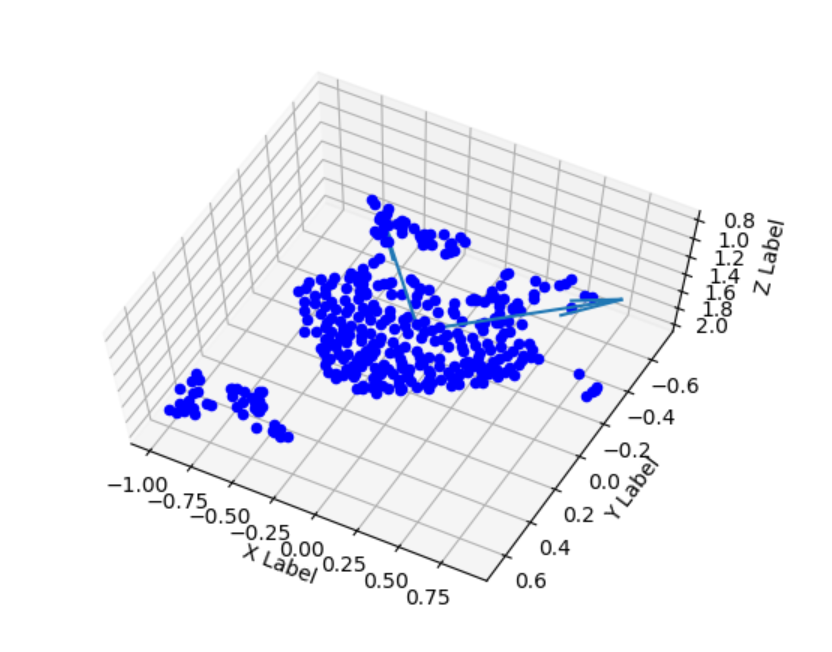
\includegraphics[width=0.9\textwidth]{images/table_automatic_axis_center_estimation.png}
        \caption{Ergebnis der automatischen Kamerakalibrierung \label{fig:camera_calibration}}
    \end{minipage}\hfill
    \begin{minipage}{0.45\textwidth}
        \centering
        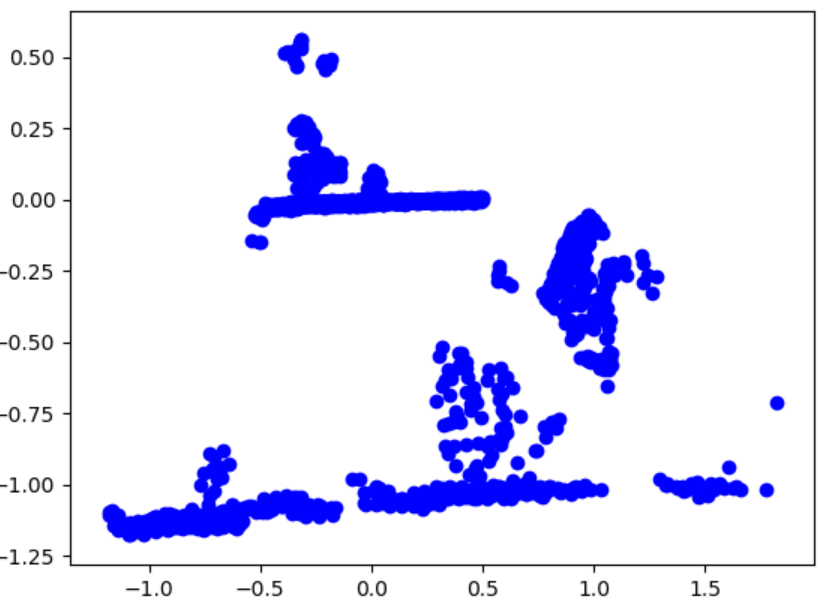
\includegraphics[width=0.9\textwidth]{images/table_manual_calibration.png}
        \caption{Oberfläche bei der manuellen Kalibrierung \label{fig:calibration_collection}}
    \end{minipage}
\end{figure} % Daniel 0.5 Seiten
\subsection{Bahnplanung \& Greifen}
\subsubsection{Bahnplanung}
Die gesamte Bahnplanungskomponente besteht aus zwei Paketen:
\begin{enumerate}
	\item \textit{cup\_acceptor\_planning}:
				\newline
				Erhält von der Highlevel-Steuerung die Posen der Tasse und des Turtlebots. Setzt Zwischenwegpunkt für die Trajektorienbestimmung. Regelt den Ablauf zwischen der Steuerung des UR5 und des PG70.
	\item \textit{cup\_acceptor\_pathing}:
				\newline
				Initialisiert MoveIt. Erhält von \textit{cup\_acceptor\_planning} eine Liste von Wegpunkten. Bestimmt mit auszuführende Trajektorie für die gegebenen Wegpunkt und führt sie auf dem UR5 aus.
\end{enumerate}
\textit{cup\_acceptor\_planning} stellt die Logik hinter der Bahnplanung dar. Sie startet Actions von \textit{cup\_acceptor\_pathing}, sowie \textit{cup\_gripper} und regelt das Zusammenspiel dieser beiden ROS-Pakete. Zunächst stellt sie sicher, dass der Roboterarm samt PG70 sich in Home-Konfiguration befinden. Danach wird zunächst der UR5 zur Tasse bewegt. Dann wird der PG70 angesteuert, um die Tasse zu greifen. Anschließend wird die Tasse zum Turtlebot geführt und dort wieder losgelassen. Letztendlich soll der Roboterarm wieder in die Home-Konfiguration zurückkehren. Für den Bahnplanungsablauf wird von \textit{cup\_acceptor\_planning} dabei neben den Posen der Tasse und des Turtlebots auch noch je ein Punkt direkt über den beiden Zielen gesetzt und zwar so, dass sich der EEF des Roboterarms einige Zentimeter über der oberen Kante der Tasse bzw. der Tischplatte befindet. \textit{cup\_acceptor\_planning} stellt eine einzige Action bereit, welche die oben beschriebene Logik ausführt. 
\newline \\
\textit{cup\_acceptor\_pathing} ist für die eigentliche Bahnplanung und Ansteuerung der Hardware mit MoveIt zuständig. Da wir die Bahnplanung in Python implementierten, mussten wir das ROS-Paket \glqq Moveit\_Commander\grqq \cite{MoveItCommander} zu unserem Projekt hinzufügen. \textit{cup\_acceptor\_pathing} erhält also eine Liste von EEF-Posen, über die es eine Trajektorie berechnen soll, welche vom UR5 ohne Kollisionen abgefahren werden kann. Dazu wird MoveIt verwendet. MoveIt stellt dabei einen kollisionsfreien Pfad sicher, da es auf unserem Modell plant, welches neben dem UR5 auch noch den PG70 samt Greiferfinger und Zwischenstück sowie den Tisch beinhaltet. Auch die IK wird von MoveIt gelöst. Es wird also online eine Abfolge von Gelenkpositionen für den UR5 bestimmt und abgefahren. \textit{cup\_acceptor\_pathing} beinhaltet dabei zwei Actions. Die \textit{plan\_and\_execute} berechnet mit \textit{compute\_cartesian\_path} über die Wegpunkt eine Trajektorie und führt sie aus, wohingegen \textit{go\_home} den Roboterarm in die Home-Konfiguration führt. Dabei wird \textit{set\_target\_pose} und \textit{plan} verwendet.
\newline \\
Die gesamte Bahnplanungskomponente besitzt dabei außerdem eine vollständige Fehlererkennung, sowie Fallback-Protokolle für die einzelnen Etappen im Ablauf. Die beiden Actions von \textit{cup\_acceptor\_pathing} können neben dem Ergebnis-Code 200 für Erfolg auch noch 500 für Misserfolg zurück liefern. In diesem Fall fängt \textit{cup\_acceptor\_planning} dies ab und weiß, dass die Bahnplanung fehlschlug. Je nachdem, in welchem Abschnitt sich der UR5 mit der Tasse befindet, wird ein dementsprechendes Protokoll abgespielt, nachdem sich der Roboterarm wieder in HOME-Konfiguration und die Tasse wieder in initialer Pose auf dem Tisch befindet. Zusätzlich stellt die Planungskomponente am Anfang der Durchführung sicher, dass sowohl die Tasse als auch der Turtlebot erreichbar ist. Dies wird einfachheitshalber über die kartesische Distanz überprüft. Sollte sich eins von beidem zu weit entfernt befinden, so wird der Ergebnis-Code 301 bzw. 302 an die Highlevel-Steuerung zurückgeliefert.
 % Robin 1 Seiten
\subsubsection{Greifen}
Die Hardware besteht aus dem Greifer Schunk PG70 mit 3D-gedruckten Fingern, die durch ein Muster aus Haushaltsgummis erweitert wurden. Die Kommunikation mit dem Greifer findet über eine CAN Schnittstelle statt, die per USB am Shuttle Computer angeschlossen ist. Ein externes Netzteil versorgt den Greifer mit Strom.

Der Greifer wird durch den \glqq schunk\textunderscore canopen\textunderscore driver\grqq des FZI angesprochen, welches eine Action zur Konfiguration der Backenabstände anbietet. Das Paket wird von \glqq cup\textunderscore gripper\grqq verwendet, ein ROS Paket mit den beiden Actionen GrabCup und ReleaseCup. GrabCup akzeptiert ein cup\textunderscore diameter als Parameter, um den Abstand der Finger auf die jeweilige Tasse anzupassen. Innerhalb des Packets wird der Greifer durch \glqq gripper \grqq abstrahiert, was einen vereinfachten Tausch der Hardware ermöglichen würde.
 % Florian 0.25 Seiten
\subsection{High-level Steuerung \& Kommunikation}
Die Highlevel Steuerung besteht aus einer Komponenten \glqq cup\textunderscore acceptor\textunderscore manager\grqq, die sowohl die Koordination der Teile innerhalb der Gruppe, als auch die Kommunikation mit dem Super Manager übernimmt. Dazu stellte diese Komponente einen Action mit dem Namen AcceptCup zur Verfügung, die nach einer erfolgreicher Bilderkennung die Tasse greift und auf den Turtlebot stellt. Dabei funktioniert die Interaktion wie folgt:
\begin{enumerate}
\item Abonnement auf Ergebnisse der Localization Komponente
\item AcceptCup Action wird aufgerufen
\item Überprüfe Bounding Boxes für Tasse und Turtlebot. Ohne Ergebnisse wird gewartet und ein Fortschritt gemeldet
\item Aufrufen der Gripper Arm Action
\item Result zurück geben
\end{enumerate}

Der besondere Augenmerk lag bei einer korrekten Kommunikation mit den anderen Gruppen, sodass der Fortschritt beim Aufrufen der Action ersichtlicht ist.
 % Yassine und Florian 0.5 Seiten

% Evaluation & Ausblick
\section{Evaluation \& Ausblick} % 2 Seiten
\subsection{Bilderkennung}
\subsubsection{Tassenerkennung}
Während die Tassenerkennung insgesamt recht robust funktioniert, gibt es durchaus noch Potential zur Verbesserung.

So könnte der für die Klassifikation der Tasse verwendete SVM Klassifikator mit variableren Trainingsdaten trainiert werden um die Generalisierung des selbigen zu verbessern und die Erkennung auch unter schwierigen bzw. varriierenden Lichtverhältnisse und mit verschiedenen Tassen robuster zu machen. Außerdem könnte der Sliding Window Ansatz, der im Moment als Standardverfahren für die Gewinnung der zu klassifizierenden Bildsegmente aktiv ist mit einem Interest Point Detektor ersetzt bzw. kombiniert werden um die Anzahl der Segmente zu reduzieren und die Erkennung damit zu beschleunigen.

Weiterer Spielraum zur Verbesserung besteht bei der Erkennung der Orientierung der Tasse. Wie beschrieben versucht der Algorithmus die Orientierung des Henkels anhand von dessen Position in der Punktwolke zu erkennen. Es stellte sich jedoch bei Tests heraus, dass der Henkel, insbesondere wenn sich die Tasse an Randpositionen des Tisches befindet, in der Punktwolke kaum auszumachen ist, weshalb die Erkennung hier häufiger versagt. Ggf. könnte man die Orientierung stattdessen mit Hilfe der Bilddaten z.B. über das Training eines Neuronalen Netzes zu realisieren. % Daniel 0.5 Seiten
\subsubsection{Turtleboterkennung}
\begin{figure}
\centering
\begin{minipage}[t]{.3\textwidth}
\centering
\vspace{0pt}
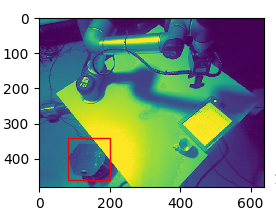
\includegraphics{./images/tb1.png}
\end{minipage}\hfill
\begin{minipage}[t]{.3\textwidth}
\centering
\vspace{0pt}
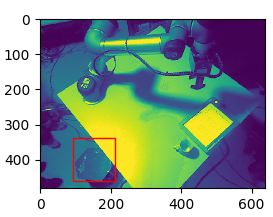
\includegraphics{./images/tb2.png}
\end{minipage}\hfill
\begin{minipage}[t]{.3\textwidth}
\centering
\vspace{0pt}
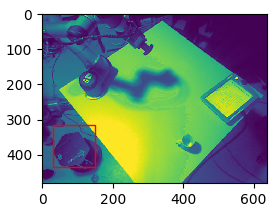
\includegraphics{./images/tb3.png}
\end{minipage}\hfill
\caption{Erkennung des Turtlebots}
\end{figure}
Der Vorteil des verwendeten Ansatzes besteht darin, dass die Erkennung des Turtlebots immer erfolgreich realisiert wird, wenn es komplett in der Szene vorkommt. Wenn aber nur ein Schnitt des Turtlebots sichtbar ist, kann es zu fehlerhaften oder ungenauen Erkennungen kommen. Dies kann verbessert werden, indem die Kamera einen größeren Bereich in Betracht zieht oder indem sie in einer anderen Position steht. Das war aber nicht möglich, weil die Hauptaufgabe der Kinect hieß, die Tasse zu erkennen.

Es ist von Nachteil, dass der Training-Datensatz unterschiedliche Lichtbedingungen nicht berücksichtigte, was die Erkennung des Turtlebots beispielsweise während der Live-Demo negativ beeinflusste. Um dies zu kompensieren, könnte eine Komponente implementiert werden, die vor der Erkennung ein Fine-Tuning des Models anhand von Szenen der neuen Umgebung realisiert, um das Model zur neuen Umständen zu adaptieren.

Darüber hinaus dauerte die Inferenz bei der Erkennung im Durchschnitt 15 Sekunden im Shuttle. Dies wurde mittels eines Parallelisierungsverfahren umgangen, was zur Folge hatte, die Inferenzzeit um 10 Sekunden (ca. 5 Sekunden/Inferenz) im Durchschnitt zu sinken. % Yassine 0.25 Seiten
\subsubsection{Automatische Kamerakalibrierung}
Generell funktioniert der beschriebene Ansatz recht robust, jedoch kommt es gelegentlich zu Fehlerkennungen bei der Detektion der Kanten des Tisches, welche zur Berechnung einer falschen Transformation vom Kamera- ins Weltkoordinaten System führen. Hier könnten weitere Überprüfungen auf die Plausibilität des Detektionsergebnisses Abhilfe schaffen.
Ein weiterer Nachteil des Ansatzes besteht darin, dass er auf den Labortisch zugeschnitten wurde. Für den Einsatz in einer anderen umgebung müsste er entsprechend angepasst werden. Ggf. wäre Alternativ eine Kalibrierung mittels eines entsprechenden Kalibrierungsobjekts bzw. Musters denkbar um die Kalibrierung flexibler zu gestalten. % Daniel 0.25 Seiten
\subsection{Bahnplanung \& Greifen}
\subsubsection{Bahnplanung}
Die erzielten Trajektorien waren für unseren Anwendungszweck annähern optimal. Zwar haben wir zwei Zwischenpunkte über den Zielen hinzugefügt, zwischen den einzelnen vorgegebenen Wegpunkte wurden allerdings die direkten Pfade gefunden und auch der Kaffee wurde dabei nicht verschüttet.
\newline
Obwohl unsere Bahnplanung vollständig zur Laufzeit stattfand, wurde die Trajektorien ohne merkbare Verzögerung berechnet und ausgeführt. Die Bahnplanung eines einzelnen Abschnittes hat dabei nie länger als 500ms für die Berechnung benötigt. Längere Verzögerungen in den Videoaufnahmen lassen sich mit der zusätzlichen Verzögerung von 500ms erklären, welche manuell eingefügt wurde, damit MoveIt genügend Zeit hat, um den momentanen Zustand des Roboterarms zu aktualisieren.
\newline \\
Bei der bisher verwendeten \textit{compute\_cartesian\_path}-Methodik gibt es jedoch einen entscheidenden Nachteil. Die Bahnplanung umfährt den Fuß des UR5 nicht eigenständig, sondern fährt gegebenenfalls den EEF über die Arm-Basis und beendet dann die Durchführung, da für die restliche Strecke keine Trajektorie mehr berechnet werden konnte. Bisher mussten wir also in manchen Situationen noch vordefinierte Umgehungspunkte hinzufügen. \textit{compute\_cartesian\_path} scheint nämlich den Arbeitsraum des UR5, welchen man ebenfalls für MoveIt anpassen kann, nicht bei der Planung zu berücksichtigen. Den Bereich über dem Roboterfuß als unzulässig zu deklarieren lieferte daher nicht den gewünschten Effekt.
\newline \\
Mit mehr Zeit würden wir als nächstes versuchen, die Bahnplanung gänzlich ohne Zwischenpunkte durchzuführen. Um dabei trotzdem die Tasse aufrecht zu halten, müsste man Pfad-Constraints hinzufügen und die Bahnplanung nur über die \textit{set\_target\_pose}-Methode durchführen.
\newline
Die so berechneten Trajektorien müssten, wie wir feststellen konnten, weiter optimiert werden, um zumindest annähernd die direkteste Bahn abzufahren. Mit der bisherigen Implementierung der \textit{set\_target\_pose}-Variante sind die Trajektorien nämlich oft noch zu ausschweifend. Da bei der Optimierung jedoch die Kinematik des Armes berücksichtigt werden muss, um die Machbarkeit zu gewährleisten und Kollisionen zu vermeiden, ist dies kein trivialer Nachbearbeitungsschritt.
\newline \\
Im bisherigen Stand der Bahnplanung ist außerdem keine Kollisionserkennung mit zusätzlichen Objekten der Umgebung implementiert. Diese Erweiterung wäre jedoch recht einfach, da das Planning Interface von MoveIt den Zustand der Szene überwacht. Könnte die Lokalisierung also für jedes Objekt auf dem Tisch und um den Tisch eine annähernd exakte Bounding Box bereitstellen, so müsste man diese nur über eine Methode zur Szene hinzufügen und schon würden sie bei der Bahnplanung mitberücksichtigt werden. Des Weiteren kann man genauso Bounding Boxen an den Roboterarm anbringen. Man könnte also auch eine Kollision der gegriffenen Tasse mit der Umgebung vermeiden. % Robin 0.5 Seiten
\subsubsection{Greifen}
Das beschriebene System wurde auf Grifffestigkeit geprüft. Dazu wurden drei unterschiedliche Ladungen einer Tasse getestet: Leer, Schrauben und Wasser (Füllstand: circa 2cm unter Rand). Die Bewegung der Tasse durch den Arm führte weder zu Verrutschen, noch zu Brechen eines Fingers. Somit kann die Tasse sicher transportiert werden, ohne Verlust des Tasseninhalts.

Jedoch bietet das implementierte System einen Nachteil: Es können nur bekannte Tassen gegriffen werden. Leider war es uns nicht möglich die Ergebnisse der Objekterkennung für eine zuverlässige Aussage über die Tassenbreite zu verwenden. Besser wäre ein Drucksensor an den Fingern oder ein anderer Greifer, der den Druck messen kann. Dieses Feedback lässt den Griff an beliebige Tassen anpassen. 
 % Florian 0.25 Seiten
\subsection{High-level Steuerung \& Kommunikation}
Zur Evaluation der Highlevel Steuerung wurden die Schnittstellen auf Funktionalität manuell getestet. Desweiteren wurden einzelne Komponenten deaktiviert, um die korrekte Rückgabe von Fehlern und Fortschritt zu prüfen. Die Verwendung eines zentralen Paketes, welches die einzelnen Schritte startet, trennt die verschiedenen Zuständigkeiten und sorgt für einen klaren Ausführungsfluss.
 % Yassine und Florian 0.25 Seiten
\subsection{Gesamtsystem}
\input{5-4_evaluation_gesamtsystem} % Daniel 0.25 Seiten

\bibliography{example}

\end{document}
